\section{Pré-processamento de Dados}
\label{sec:data-preproces}

Uma vez determinada a tarefa a ser realizada, deve\hyp{}se analisar os dados que serão utilizados, com o objetivo de averiguar se estão estruturados de maneira que permitam a maior eficiência do algoritmo de mineração escolhido. Bases de dados reais, ao redor do mundo, podem não garantir essa eficiência desejada, devido a presença de fatores negativos que atuam sobre os dados e podem impossibilitar o algoritmo de obter padrões representativos a partir destes dados

Para tal, a etapa de pré\hyp{}processamento de dados se faz necessária. Este processo é definido por \citeonline{garcia2015data} como um conjunto de técnicas que inicializam os dados de maneira que estes sirvam como entrada para certos algoritmos de mineração. As técnicas dividem-se em dois tipos: técnicas de preparação de dados e técnicas de redução de dimensionalidade.

Durante a etapa de pré\hyp{}processamento ocorre a conversão dos dados que são considerados inúteis ao algoritmo escolhido, em dados que possam ser utilizados. Isto pode provocar a aceleração da fase de mineração, o que faz do pré\hyp{}processamento uma etapa obrigatória para a descoberta de conhecimento.

De acordo com \citeonline{larose2014discovering}, o pré\hyp{}processamento se faz necessário devido a quantidade de dados incompletos, não processados e ruidosos que existe em algumas bases. Podendo conter: i) \textit{outliers}; ii) dados em formatos diferentes daqueles aceitos pelo algoritmo de mineração a ser executado; ou iii) campos obsoletos ou redundantes. Portanto, a aplicação de técnicas de pré\hyp{}processamento pode aumentar a precisão e eficiência dos algoritmos de mineração utilizados sobre estes dados.

\subsection{Preparação de Dados}
\label{subsec:data-prep}

Técnicas de preparação têm por objetivo a limpeza e conversão de dados. \citeonline{bramer2007principles} observa que a tarefa mais complexa para algumas aplicações é a padronização dos dados para análise. Esta padronização acontece no decorrer do processo de transformação de dados. Compõem a preparação técnicas de:

\begin{enumerate}[label=\roman*.]
    \item Limpeza de dados {--} Busca a correção, filtrando dados incorretos e reduzindo detalhamento desnecessário, bem como, tratando valores faltosos e identificando ruídos;
    \item Transformação de dados {--} Converte os dados para que sejam utilizados de maneira mais eficiente pela tarefa de mineração escolhida, incluindo técnicas de construção de atributos, agregação e normalização de dados;
    \item Integração de dados {--} Unifica múltiplas fontes de dados, evitando redundâncias e inconsistências na base final.
\end{enumerate}
Estas são técnicas importantes para garantir a precisão, integridade e consistência dos dados.

\subsection{Limpeza de Dados}
\label{subsec:data-clean}

Bases reais podem conter dados impróprios, incompletos ou inesperados. A aplicação de um processo de mineração sobre uma base que contenha uma quantidade relativamente alta destes dados pode resultar em um modelo de representação inválido. Estes dados impactam o resultado de maneiras diferentes, dependendo diretamente do algoritmo utilizado \cite{han2000data}.

Um dos tipos de dados inesperados comumente encontrados em bases de dados são os valores errados. Tratados como ruídos, estes serão estudados detalhadamente na Seção \ref{subsubsec:noise}. Dados errados são categorizados por \citeonline{bramer2007principles} entre valores possíveis e impossíveis ao atributo. Na primeira categoria encontram\hyp{}se por exemplo, números como 60.50 que pode ser armazenado como 6.050, ou valores categóricos (preto sendo armazenado como verde). Enquanto na segunda categoria podem ser observados exemplos como 6M50 ao invés de 6.050. Percebe-se então que a primeira aborda valores válidos, enquanto na segunda encontram\hyp{}se os valores inválidos.

\begin{figure}[H]
    \centering
    \caption{Base de dados antes da limpeza.}
    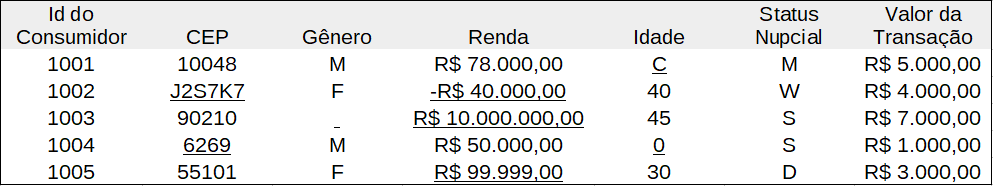
\includegraphics[width=\linewidth]{figuras/dirty-base.png}
    \source{Adaptado de \cite{larose2014discovering}.}
    \label{fig:data-before-cleaning}
\end{figure}

Exemplos de dados impróprios, tanto válidos quanto inválidos, podem ser encontrados na Figura \ref{fig:data-before-cleaning}. Nesta amostra de dados comercial podem ser encontrados valores inesperados, porém válidos, como o CEP e idade do consumidor 1004, bem como valores inválidos, como a idade do consumidor 1001.

Os erros destacados na Figura \ref{fig:data-before-cleaning} podem ocorrer devido a falhas na entrada, atualização ou transmissão de dados, assim como durante a etapa de integração de dados. A localização de erros é fácil para um conjunto reduzido de dados como aquele mostrado na Figura \ref{fig:data-before-cleaning}, porém, o mesmo pode não ocorrer para as bases de dados reais que podem conter diversos atributos e incontáveis instâncias.

\subsubsection{Valores Faltosos}
\label{subsubsec:missing-values}

Em todas as bases de dados reais há potencial para a existência de valores faltosos, que podem ocorrer devido aos mais diversos motivos. Mesmo em grandes conjuntos de dados, o subconjunto de instâncias com dados completos pode ser relativamente pequeno. Embora alguns métodos de mineração obtenham resultados satisfatórios ao utilizarem dados contendo valores faltosos, outros necessitam integridade nas instâncias analisadas. A resposta mais simples para lidar com estes valores faltosos é a eliminação, o que, dependendo do tamanho da base de dados, pode não ser a melhor solução \cite{kantardzic2011data}.

\begin{figure}[H]
    \centering
    \caption{Base \textit{cars} contendo valores faltosos.}
    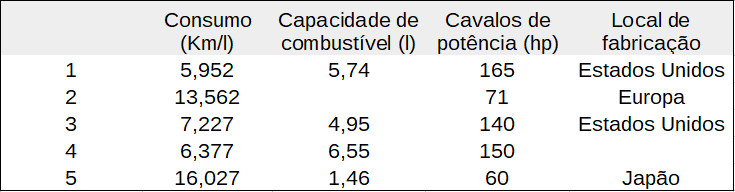
\includegraphics[width=\linewidth]{figuras/cars-missing-values.png}
    \source{Adaptado de \cite{larose2014discovering}.}
    \label{fig:cars-missing-values}
\end{figure}

A amostra de dados representada na Figura \ref{fig:cars-missing-values}, constituída de informações sobre carros produzidos entre os anos de 1970 e 1980, é um exemplo de base de dados contendo valores faltosos. Em contrapartida a resposta padrão das ferramentas, \citeonline{larose2014discovering} utiliza uma base de dados para mostrar o funcionamento das técnicas mais comumente utilizadas ao lidar com estes valores. As técnicas mostradas pelos autores foram:

\begin{enumerate}[label=\roman*.]
    \item Substituir o valor por uma constante determinada pelo analista, conforme apresentado na Figura \ref{fig:cars-labels};
    \item Substituir o valor pela média aritmética do campo (para valores numéricos) ou a moda (para valores categóricos);
    \item Substituir os valores faltosos por um valor gerado aleatoriamente a partir da distribuição observada na variável;
    \item Substituição por inserção de valores, gerando novos valores com base em outras características do exemplo.
\end{enumerate}

\begin{figure}[H]
    \centering
    \caption{Base \textit{cars} com valores faltosos substituidos por constantes.}
    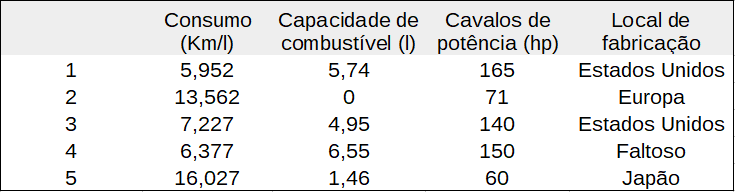
\includegraphics[width=\linewidth]{figuras/cars-constants.png}
    \source{Adaptado de \cite{larose2014discovering}.}
    \label{fig:cars-labels}
\end{figure}

O valor numérico para substituição por média pode ser obtido através da equação (\ref{eq:2.1}).

\begin{equation}
    valor = \left ( \frac{\sum_{i=1}^{n} v_i}{n} \right )
    \label{eq:2.1}
\end{equation}
onde: $v_i$ corresponde ao $i$-ésimo valor do atributo $v$ e $n$ representa o total de instâncias da base, enquanto valores categóricos podem ser substituídos por popularidade ou moda, onde os valores de maior ocorrência para atributo em questão são utilizados para preencher os dados faltosos. Ambas as abordagens podem ser observados na Figura \ref{fig:cars-mean-trend}.

\begin{figure}[H]
    \centering
    \caption{Base \textit{cars} com valores substituídos por média e moda.}
    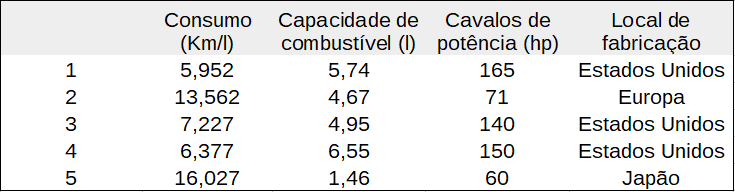
\includegraphics[width=\linewidth]{figuras/cars-mean-trend.png}
    \source{Adaptado de \cite{larose2014discovering}.}
    \label{fig:cars-mean-trend}
\end{figure}

Outra abordagem para a correção de valores faltosos é a inserção. Esta utiliza modelos de predição através de regressão múltipla, fazendo uso de variáveis existentes a fim de estimar um valor para o dado faltoso (\textit{e.g.} para a base \textit{cars}, mostrada na Figura \ref{fig:cars-missing-values}, utilizar os atributos cavalos de potência e capacidade de combustível para estimar o consumo). Valores gerados por inserção apresentam maior precisão. O modelo de predição é criado baseando\hyp{}se no nível de correlação entre os atributos \cite{larose2014discovering, osborne2012best, refaat2010data}.

\subsubsection{Suavização de Ruídos}
\label{subsubsec:noise}

Assim como ocorre com os valores faltosos, a presença de ruídos pode afetar a interpretação dos dados, os modelos criados a partir destes dados e as decisões tomadas a partir da interpretação e dos modelos. Ruídos são definidos por \citeonline{han2000data} como um erro aleatório ou variância em uma variável e são amplamente estudados em exemplos de classificação e regressão, onde sua presença dificulta a extração de conhecimento, pois podem causar perturbação nos limites de classes, aumentando a sobreposição entre elas. \citeonline{garcia2015data} listam as abordagens mais importantes ao lidar com dados ruidosos, são elas:

\begin{enumerate}[label=\roman*.]
    \item Algoritmos robustos {--} O nível de robustez de um algoritmo é determinado pela influência que o ruído exerce sobre ele. Algoritmos robustos são menos influenciáveis, possibilitando maior precisão nos resultados;
    \item Métodos de polimento de dados {--} Estas técnicas buscam corrigir instâncias ruidosas antes do treinamento de algum algoritmo. Isto é viável apenas para conjuntos pequenos de dados visto que, geralmente, consomem muito tempo;
    \item Filtros de ruído {--} Identificam elementos que possam ser eliminados da base de treinamento. Esta é a abordagem mais utilizada pois, como discutido na Seção \ref{subsubsec:missing-values}, é a resposta padrão dos algoritmos de mineração que tratam anomalias nos dados.
\end{enumerate}

Alguns dos métodos de polimento são apresentados por \citeonline{han2011data}, entre eles encontram-se: a suavização por cesto (\textit{binning}) e regressão. A primeira suaviza valores baseando-se em seus vizinhos, os elementos mais próximos a ele, sorteando\hyp{}os em cestos, enquanto a segunda utiliza regressão linear ou multilinear para encontrar o valor adequado, baseando\hyp{}se em outros atributos do elemento. Algumas técnicas de \textit{binning} estão representadas na Figura \ref{fig:binning}, onde os valores foram divididos em cestos de tamanho único, definido pelo usuário da técnica, a quantidade de cestos é dada pela equação (\ref{eq:2.2}).

\begin{equation}
    cestos = \frac{n}{x}
    \label{eq:2.2}
\end{equation}
onde: $n$ corresponde ao número de itens na base e $x$ a quantidade de itens que deve existir em cada cesto.

Os valores nos cestos podem ser suavizados utilizando a média, limite dos valores ou técnicas de regressão. Na suavização por média, cada valor é substituído pela média do grupo ao qual pertence, que pode ser obtida através da equação \ref{eq:2.1}. A técnica que usa limites identifica o menor e maior valor do cesto como seus limites superior e inferior e os elementos são substituídos por aquele ao qual mais se aproxima. O método de regressão envolve o uso de regressão linear ou multilinear para estimar o valor a ser inserido.

\begin{figure}[H]
    \centering
    \caption{Técnicas de suavização por cesto.}
    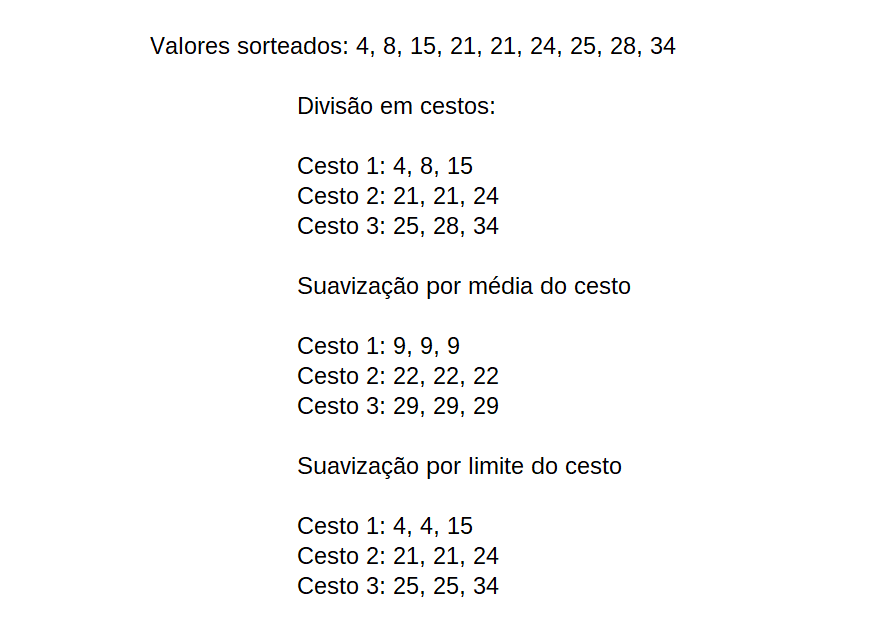
\includegraphics[width=0.9\linewidth]{figuras/binning.png}
    \caption*{Fonte - Adaptado de \cite{han2000data}.}
    \label{fig:binning}
\end{figure}

\subsection{Detecção de Anomalias}
\label{subsec:outliers}

Segundo \citeonline{romero2014survey}, detecção de anomalias, ou \textit{outliers}, é o processo de encontrar instâncias significantemente diferentes do restante dos exemplos na base de dados em que está inserida. A Figura \ref{fig:outliers} apresenta este conceito, os elementos na área \textit{R} possuem comportamento diferente do restante do grupo.

\textit{Outliers} são analisados de maneira diferente daquela utilizada para ruídos. Enquanto o último representa erros nos dados armazenados e é alvo de técnicas corretivas, o primeiro compreende exemplos válidos a observação. Estas anomalias são organizadas por \citeonline{han2011data} em três grupos, são eles:

\begin{enumerate}[label=\roman*.]
    \item Anomalias globais {--} Também conhecidos como anomalias pontuais, são as instâncias que mais se afastam do restante do conjunto em que estão inseridas, um exemplo é observado na Figura \ref{fig:outliers};
    \item Anomalias contextuais {--} Diferente dos exemplos globais, para que dados sejam categorizados como anomalias contextuais deve existir dependência com uma ou mais informações acerca dos dados (\textit{e.g.} uma temperatura elevada pode ser considerada como anomalia se ocorrer durante o inverno). O atributos avaliados são agrupados entre: contextuais e comportamentais;
    
    \begin{figure}[H]
        \centering
        \caption{Amostra de \textit{outliers}.}
        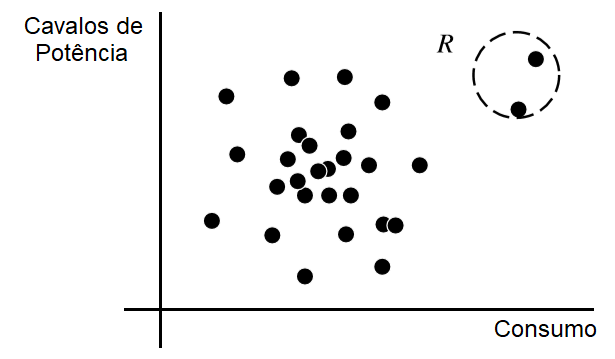
\includegraphics[width=0.7\linewidth]{figuras/outliers.png}
        \caption*{Fonte - Adaptado de \cite{han2011data}.}
        \label{fig:outliers}
    \end{figure}
    
    \item Anomalias coletivas {--} Caracterizam\hyp{}se como anomalias coletivas subconjuntos na base de dados que, quando observados individualmente, poderiam não seriam considerados anomalias. Um exemplo pode ser observado ao analisar atrasos no envio de cargas. Individualmente os atrasos podem não ser considerados como anomalias, porém, diversas ocorrências podem caracterizar uma anomalia coletiva.
\end{enumerate}

Em \citeonline{osborne2012best}, o autor utiliza distribuição normal, observada na equação (\ref{eq:2.3}), para detecção de \textit{outliers}.

\begin{equation}
    y = \frac{1}{\sqrt{2\pi}}{e^{\frac{-x^{2}}{2}}}
    \label{eq:2.3}
\end{equation}
onde: $x$ corresponde a distância, em desvios padrão, do meio e $e$ representa a constante de Euler (2.71828...). A distribuição normal é utilizada pelo fato de ser conhecido a porcentagem da população estudada que encontra-se em dado ponto da distribuição. Assim, é possível identificar a possibilidade de um elemento estar situado fora de um desvio padrão aceitável.

O autor estabelece este padrão em +/-3.0, pois, de acordo com o método utilizado, cerca de 0,26\% da população encontra-se além deste limite. As instâncias com desvio próximo a esse número são definidos como \textit{fringeliers}, exemplos que possuem comportamento anormal, porém, menos aparente e as instâncias que apresentam desvio padrão superior ao limite estabelecido são denominados \textit{outliers}.

\subsection{Redução de Dimensionalidade}
\label{subsec:data-reduction}

Técnicas de redução de dimensionalidade buscam remover ou agrupar dados ao longo dos atributos e exemplos que compõem o conjunto trabalhado. Segundo \citeonline{kantardzic2011data}, estas técnicas são necessárias quando o objeto de estudo contém um alto número de atributos, pois a aplicação de algoritmos de mineração nestas bases possivelmente demandariam um alto custo computacional e diminuiria a eficiência do processo de descoberta de conhecimento.

De acordo com \citeonline{garcia2015data}, o maior problema de mineração de dados em grandes bases é a grande quantidade de variáveis que podem influenciar diretamente a predição. A alta dimensionalidade dos conjuntos de entrada para estes algoritmos aumenta exponencialmente o espaço de busca, além da possibilidade de obter um modelo inválido a partir do processo empregado. Os autores dividem as técnicas de redução em categorias como:

\begin{enumerate}[label=\roman*.]
    \item Seleção de atributos {--} Tem por objetivo diminuir a quantidade de atributos da base por meio de remoção ou agregação;
    \item Seleção de instâncias {--} Busca substituir o conjunto original de dados por uma versão alternativa, reduzida, dos mesmos.
\end{enumerate}

\subsubsection{Seleção de Atributos}
\label{subsubsec:atribute-selection}

A alta dimensionalidade de bases de dados é um obstáculo a ser contornado durante a descoberta de conhecimento. Segundo \citeonline{liu2012feature}, a seleção de atributos, conhecida como \textit{feature selection}, é uma técnica importante utilizada para superar este obstáculo. O resultado obtido após a seleção é um conjunto reduzido dos atributos originais e a necessidade da aplicação desta técnica pode variar, desde a melhora de performance dos algoritmos de mineração utilizados até a remoção de ruídos.

De acordo com \citeonline{borges2006reduccao}, a seleção de atributos é um processo cujo objetivo é descobrir um subconjunto de atributos relevantes para uma tarefa, considerando os dados originais. Os subconjuntos são criados baseando-se em critérios, que podem estar relacionados desde o nível de acurácia que os atributos proporcionam até um número fixo determinado pelo usuário (\textit{e.g.} três atributos).

Segundo \citeonline{garcia2015data}, seleção destes subconjuntos pode ser considerada como um problema de busca, cada estado do espaço de busca corresponde a um subconjunto de atributos. As buscas por atributos numa base ocorre nas seguintes direções:

\begin{enumerate}[label=\roman*.]
    \item Para frente (\textit{sequential forward generation} {--} SFG) {--} Inicia com um conjunto vazio e adiciona atributos até que obtenha um conjunto completo ou que o melhor subconjunto seja escolhido;
    \item Para trás (\textit{sequential backward generation} {--} SBG) {--} Ao contrário de SFG, inicia de um conjunto completo e remove atributos;
    \item Bidirecional (\textit{bidirectional generation} {--} BG) {--} Assumindo que o melhor subconjunto de atributos encontra-se entre os conjuntos vazio e cheio, é aplicado SFG e SBG em paralelo.
\end{enumerate}

O critério de escolha atua informando qual o atributo à ser adicionado ou removido do subconjunto. \citeonline{kantardzic2011data} utiliza o coeficiente de correlação de Pearson, apresentada na Equação \ref{eq:pearson-corr}, para avaliar atributos de acordo com a dependência existente entre o alvo da avaliação (\textit{i.e.} classe) e o atributo testado, candidato a compor o subconjunto.

\begin{equation}
    P\left ( x,y \right ) = \frac{\sum_{i=0}^{n}\left ( x_i-{x}' \right )\left ( y_i-{y}' \right )}{\left [ \sum_{i=0}^{n}\left ( x_i-{x}' \right )^{2} \sum_{i=0}^{n}\left ( y_i-{y}' \right )^{2} \right ]}
    \label{eq:pearson-corr}
\end{equation}
onde: $i$ corresponde ao $i$-ésimo valor dos atributos $x$ e $y$ e os termos $x^{'}$ e $y^{'}$ representam as médias de $x$ e $y$. Embora este método possa detectar apenas dependências lineares e sua utilização possa levar à seleção de atributos redundantes, o autor cita que mesmo estes atributos, quando observados em conjunto, podem fornecer informações importantes.

\subsubsection{Seleção de Instâncias}
\label{subsubsec:instance-selection}

Técnicas de seleção de instâncias, também conhecidas como amostragem (do inglês, \textit{sampling}), possuem propósito semelhante àquele da seleção de atributos, a melhora de desempenho em algoritmos de mineração através da redução do conjunto de dados a ser utilizado. Então, \citeonline{han2011data} definem \textit{sampling} como técnicas de redução que permitem uma grande quantidade de dados ser representada por uma amostra consideravelmente menor, obtida a partir do conjunto original e de forma aleatória.

As técnicas de amostragem comumente utilizadas para atingir o objetivo de redução de dados podem ser observadas na Figura \ref{fig:sampling}, onde é representado uma base $D$ que contém $N$ instâncias. As técnicas citadas são:

\begin{enumerate}[label=\roman*.]
    \item Amostra aleatória simples sem substituição de tamanho (SRSWOR) {--} Seleciona $n$ das $N$ instâncias presentes em $D$, onde $\left ( n < N \right )$. Todos os exemplos possuem a mesma probabilidade de serem escolhidos para constituírem o conjunto $n$;
    
    \begin{figure}[H]
        \centering
        \caption{Técnicas de \textit{sampling}.}
        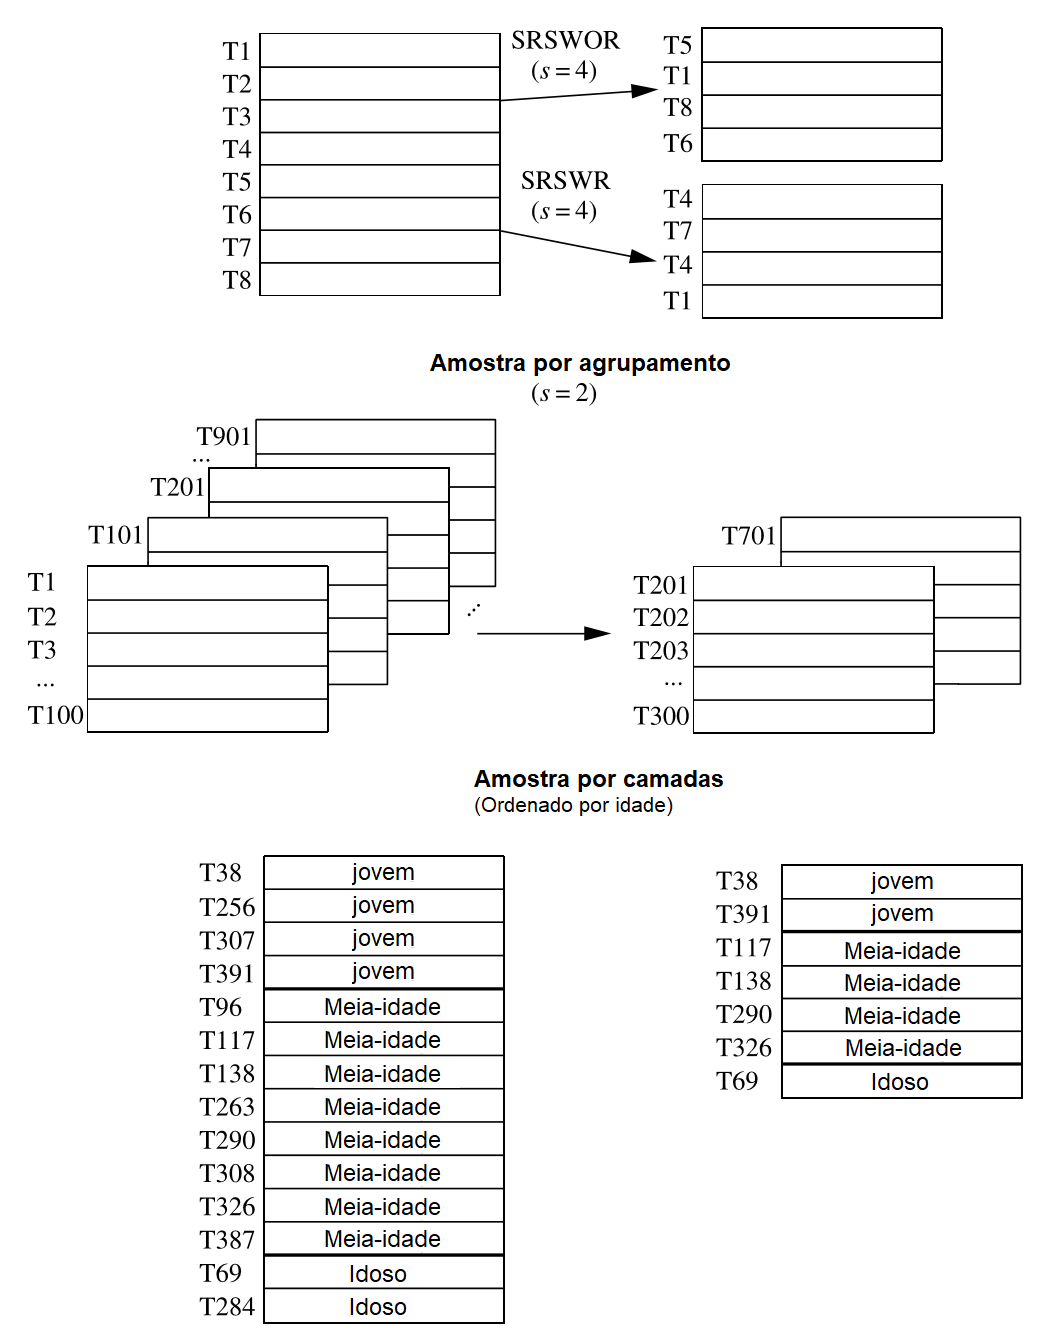
\includegraphics[width=0.65\linewidth]{figuras/sampling.png}
        \source{Adaptado de \cite{han2011data}.}
        \label{fig:sampling}
    \end{figure}
    
    \item Amostra aleatória simples com substituição de tamanho (SRSWR) {--} Possui execução similar ao SRSWOR, porém, ao selecionar um exemplo para o novo conjunto ($n$), o mesmo pode ser selecionado novamente;
    \item Amostra de agrupamento {--} Caso os dados contidos na base $D$ estejam organizados em agrupamentos mutuamente excludentes. É aplicado uma das técnicas anteriores para obter amostras dos \textit{clusters} individuais;
    \item Amostragem em camadas {--} Similar a técnica de amostragem por agrupamentos, esta utiliza SRSWOR ou SRSWR para obter amostras dos dados divididos em camadas. Estas camadas podem ser compostas de pessoas de mesma faixa etária. Desta maneira, todas as camadas serão representadas no conjunto final.
\end{enumerate}

Os autores em \cite{garcia2015data} discordam da forma de execução da amostragem, não a considerando como seleção de instâncias devido ao seu método de seleção aleatório. Segundo os autores, deve ocorrer a aplicação de critérios de escolha para os exemplos que irão compor a base final.

De acordo com \citeonline{olvera2010review}, em similaridade a seleção de atributos, os métodos para escolha de instâncias podem ser divididos entre duas categorias: i) embrulho (\textit{wrapper}), onde o critério de seleção é baseado na precisão obtida pelo classificador utilizado; e ii) filtro, aqueles em que é utilizada uma função como critério de seleção, tornando\hyp{}a independente do classificador. Os métodos de filtro tem como foco identificar e remover instâncias de borda, aquelas que pertencem a uma classe, porém, são classificadas de maneira diferente devido a semelhança com outros exemplos. A remoção das instâncias de borda preservam as margens das classes, facilitando a tarefa de classificação. Dados podem ser descartados baseando-se no conceito de fraqueza, um valor baseado na distância entre o exemplo analisado e uma instância de classe diferente, respeitando os valores dos atributos.